\section{SWID Erweiterung}
\section{Datenmodell}
\begin{figure}[H]
\centering
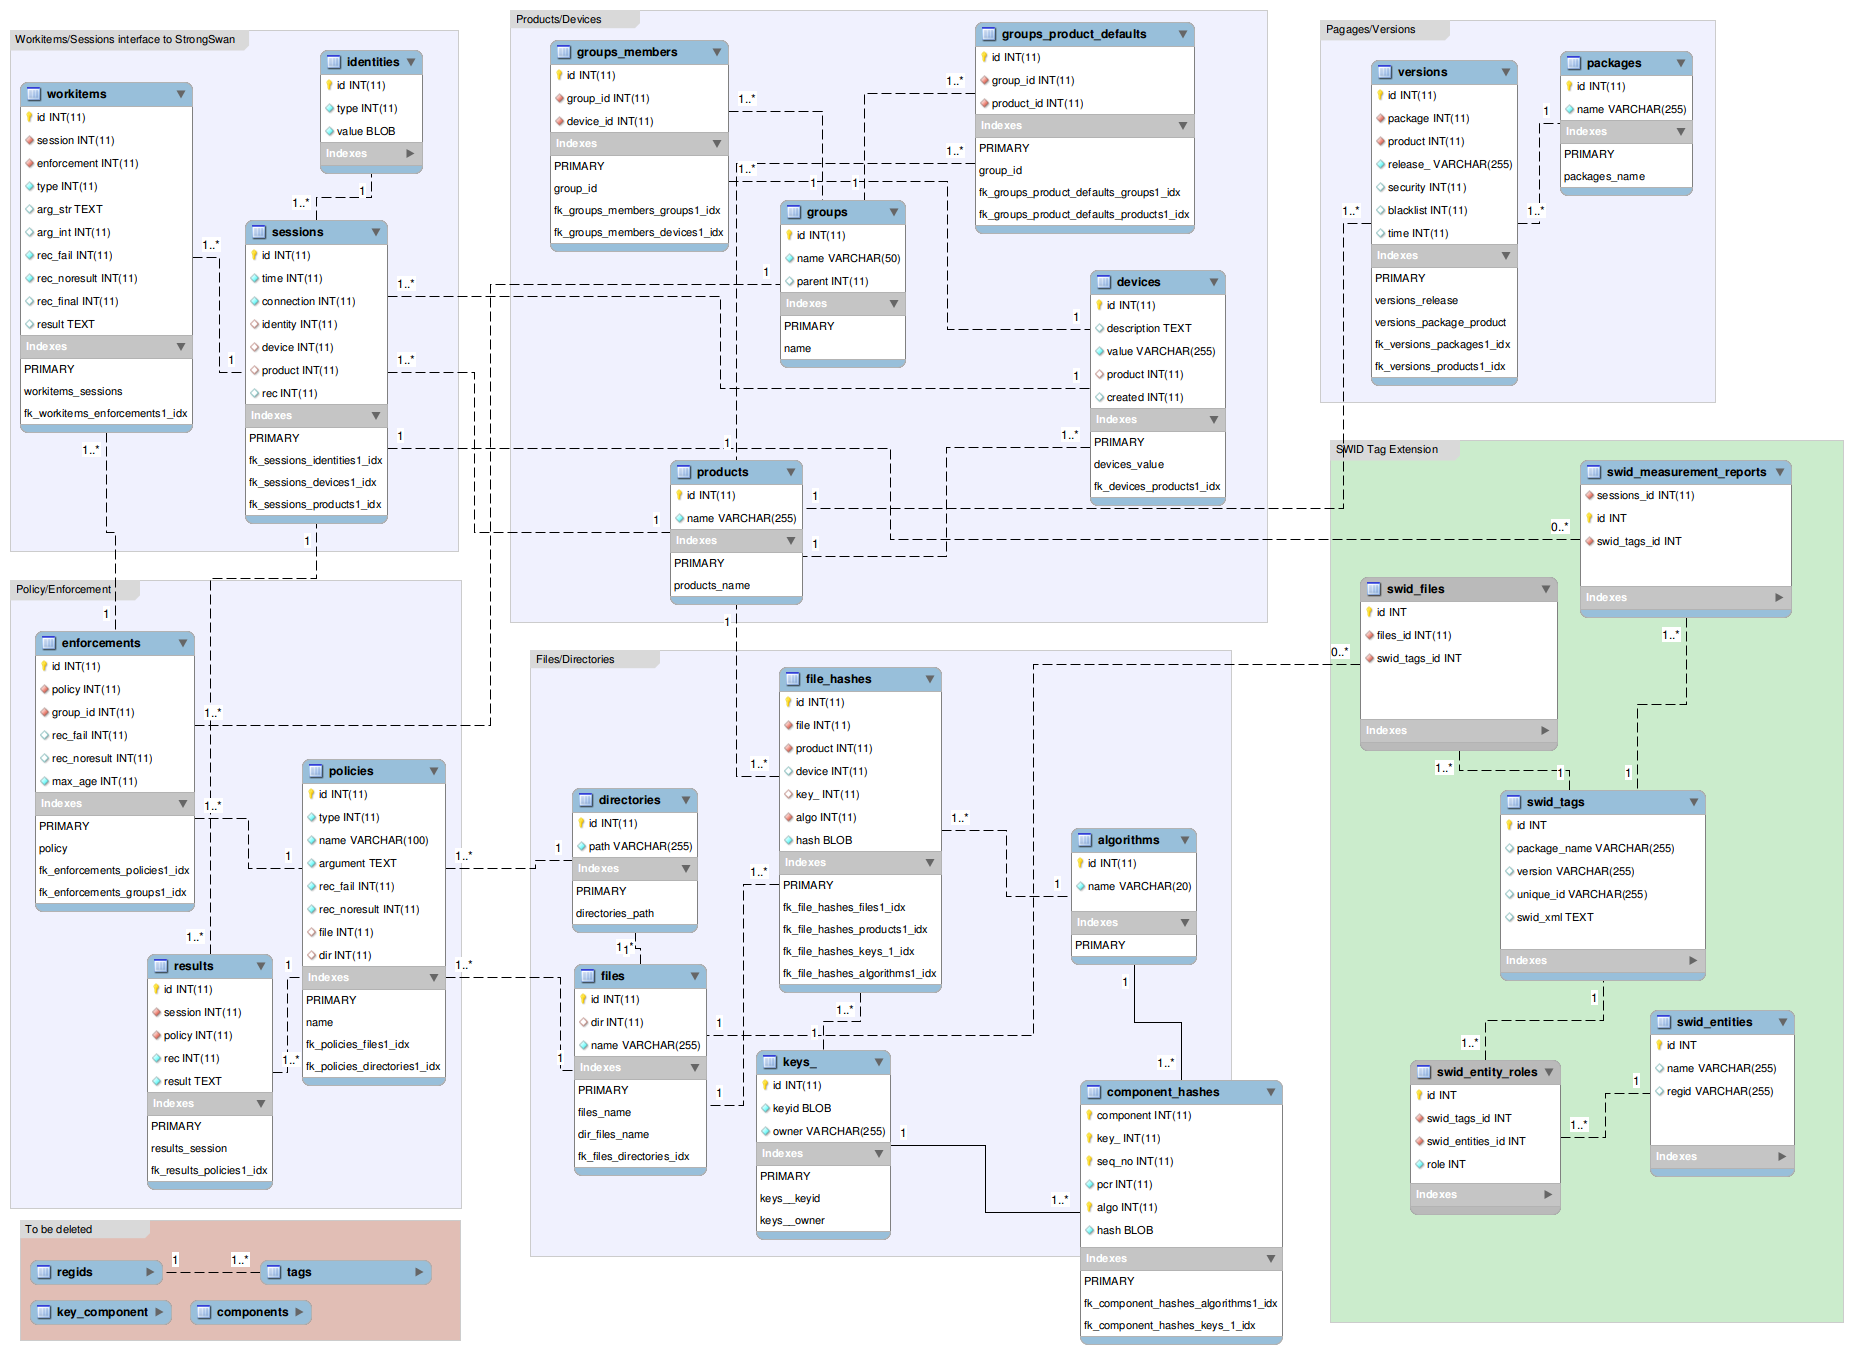
\includegraphics[angle=90,width=0.8\textwidth]{./images/db/database-model}
\caption{Bestehendes Datenmodel inklusive SWID Erweiterung (grün)}
\label{fig:database-model}
\end{figure}
Die Erweiterung des bestehenden Datenmodells ist in \autoref{fig:database-model} zu sehen. Die hinzugefügten Tabellen sind durch den grünen Hintergrund hervorgehoben. Bei Tabellen mit grauem Rahmen handelt es sich um Zwischentabellen, welche eine N zu M Beziehung auflösen. Beim modellieren der zusätzlichen Tabellen wurde darauf geachtet, dass keine bestehenden Tabellen angepasst werden mussten. Die Beziehungen werden daher alle von der Seite der Erweiterung hergestellt.
\begin{description}
\item [swid\_entityroles] Ein SWID Tag kann mehrere Entities enthalten. Entities haben nehmen in einem Tag eine oder eine Kombination von Rollen ein. Es existieren die Rollen Tag Creator, Licensor und Publisher. Pro SWID Tag darf es allerdings nur einen Tag Creator geben. Dieser Constraint wird jedoch erst in den Django Models durch das \gls{ORM} angewandt.

\item [swid\_tags\_files] In dieser Tabelle wird die Beziehung zwischen einem File und einem SWID Tag festgehalten. Ein SWID Tag kann mehrere Files beinhalten (\nameref{strongTNC:UC04}).

\item[swid\_tags\_sessions] Beim Durchführen einer Messung von SWID Tags werden die entsprechenden Tags in dieser Tabelle abgespeichert (\nameref{strongTNC:UC06}). Im dieser Tabelle werden die gemessenen Tags mit passenden Session verknüpft.

\item[swid\_entity] 
Diese Tabelle beinhaltet alle erfassten Entities. In der Regel ist eine kleine Anzahl unterschiedlicher Entities zu erwarten, weshalb diese in einer eigenen Tabelle gehalten werden und über die swid\_entityroles mit den SWID Tags verknüpft werden.

\end{description}

\section{Architektur SWID Messung}
\begin{figure}[H]
\centering
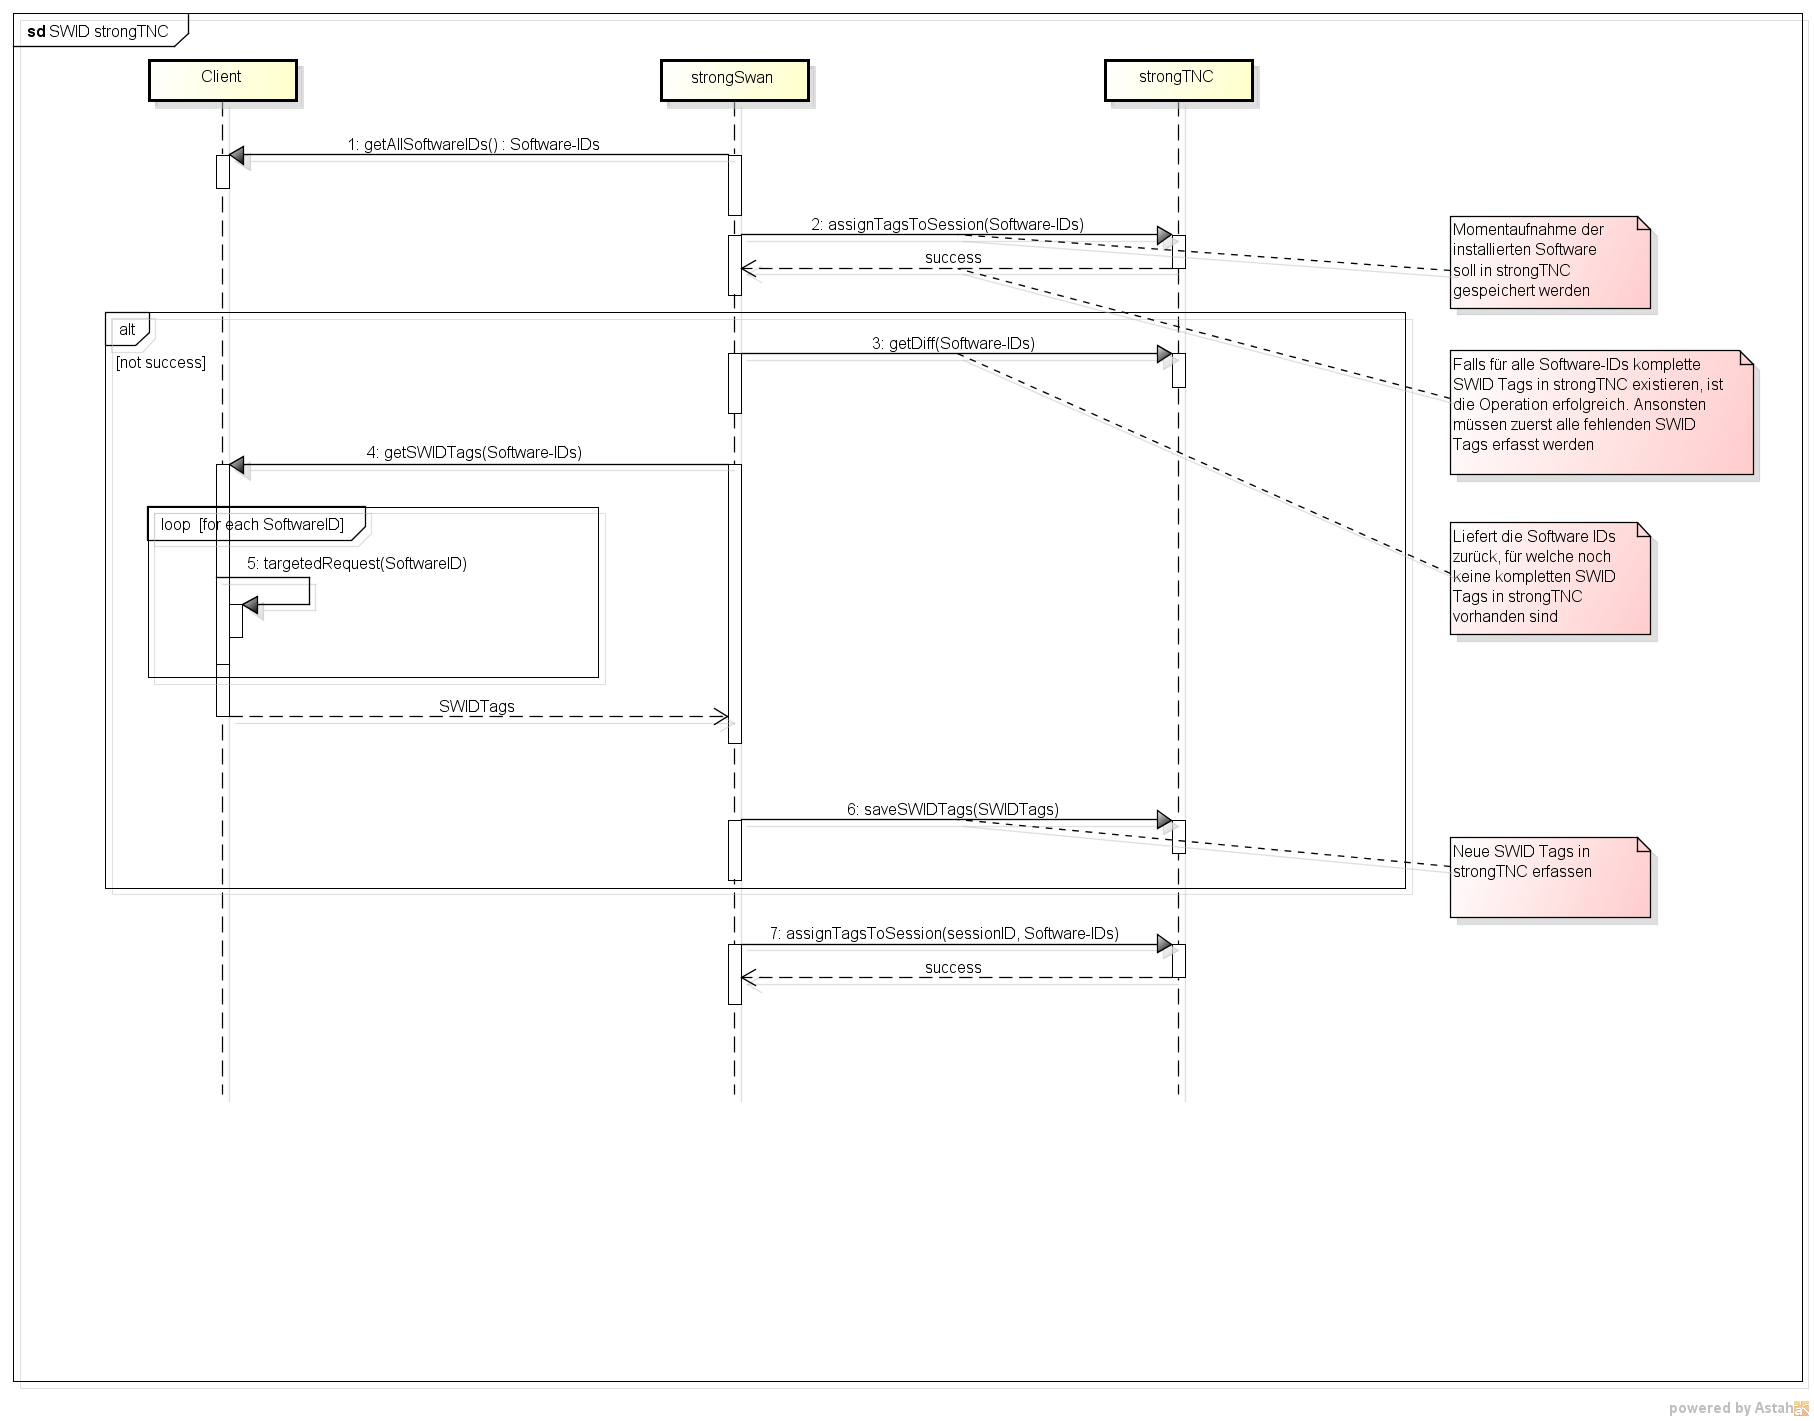
\includegraphics[width=0.9\textwidth]{./images/architecture/SWID_strongTNC.png}
\caption{Ablauf SWID Tag Messung eines Gerätes}
\label{fig:swid-measurement}
\end{figure}
In \autoref{fig:swid-measurement} ist der Ablauf der SWID Tag Messung (\nameref{strongTNC:UC06}) ersichtlich.
Eine Messung läuft wie folgt ab:
\begin{enumerate}
\item Auf dem Client werden die Software-IDs aller installierten Pakete generiert. 
\item Es wird versucht die Liste der generierten Software-IDs mit einer Session zu verknüpfen.
	\begin{itemize}
	\item Existiert zu allen Software-IDs ein entsprechender SWID Tag, ist die Messung abgeschlossen und die SWID Tags sind mit der Session verknüpft. ENDE
	\item Existiert für mindestens eine Software-ID kein entsprechender SWID Tag, wird die Messung abgebrochen und eine Liste jener Software-IDs, für welche kein SWID Tag existiert, zurückgeliefert. Weiter zu Punkt 3.
	\end{itemize}
\item Bevor die Messung durchgeführt werden kann, müssen die fehlenden SWID Tags erfasst werden. Die einzelnen XML Dokumente der SWID Tags werden vom Client anhand sogenannter \enquote{Targeted Requests} (TODO Referenz swidgenerator) erstellt, das heisst, der Generator kreiert gezielt die Tags für die gegebenen Software-IDs und nicht für alle installierten Software Pakete.
\item Der Client erfasst alle neu generierten SWID Tags in strongTNC.
\item Der Client startet erneut eine Messung und übermittelt nochmals alle Software-IDs. Nun sind für alle Software-IDs die entsprechenden SWID Tags vorhanden und die Messung wird erfolgreich abgeschlossen. Ansonsten weiter zu Schritt 2.
\end{enumerate}
Dieses Vorgehen erzwingt eine Aktualisierung der strongTNC Datenbank wenn diese nicht alle SWID Tags enthält, bevor eine Messung erfolgreich abgeschlossen werden kann. Dadurch wird erreicht, dass auf Serverseite kein Zustand gewahrt werden muss, wie es für eine nicht abgeschlossene Messung, welche später abgeschlossen wird, der Fall wäre. Dieses Vorgehen entspricht den Prinzipien von HTTP, eine Messung kann jederzeit durchgeführt werden ohne das ein Zustand oder Kontextinformationen vorhanden sein müssen. Das heisst, wenn eine Messung nicht vollständig und korrekt durchgeführt werden kann, werden keine Daten verändert. 



\subsection{Technische Umsetzung}
Der Zugriff auf die beschriebene Systemoperation erfolgt durch die, in dieser Arbeit ausgearbeiteten, RESTful HTTP Schnittstelle. Das komplette Konzept ist in (TODO Referenz REST Konzept) zu finden.

\subsubsection{REST Kommunikation}
Im Folgenden soll der Ablauf einer Messung anhand eines konkreten Beispiels illustriert werden.
In diesem Beispiel soll eine Messung für 3 Tags mit folgenden Software-IDs erfolgen:
\begin{textcode}
regid.2004-03.org.strongswan Ubuntu 12.04-i686-logrotate-3.7.8-6ubuntu5
regid.2004-03.org.strongswan Ubuntu 12.04-i686-lsb-base-4.0-0ubuntu20
regid.2004-03.org.strongswan Ubuntu 12.04-i686-strongswan-4.5.2-1.5+deb7u3
\end{textcode}

Der HTTP/REST Endpunkt wurde wie folgt definiert:
\begin{mdframed}[style=def]
\begin{description*}
	\item[URI Path] \texttt{/products/}
	\item[Archetype] Collection
	\item[Methods] GET, POST
	\item[JSON Format Response] \hfill
	
\begin{jsoncode}
{"data" : 
	[
	"software-ids TODO vom api konzept kopieren!" 
	]
}
\end{jsoncode}
\end{description*}
\end{mdframed}



\subsubsection*{Übermitteln von Software-IDs}
Die Daten werden als JSON-Liste an den entsprechenden Endpoint gesendet.
Der HTTP Request sieht folgendermassen aus:

\begin{listing}
\caption{Übermitteln von Software-IDs via HTTP/REST API}
\begin{httpcode}
POST /api/sessions/2/swid-measurement/ HTTP/1.1
Authorization: Basic cm9vdDpyb290
Host: tncserver:8000
Accept: application/json
Content-Type: application/json; charset=utf-8
Content-Length: 232

{
	"data":
	[
		"regid.2004-03.org.strongswan_Ubuntu_12.04-i686-logrotate-3.7.8-6ubuntu5",
		"regid.2004-03.org.strongswan_Ubuntu_12.04-i686-lsb-base-4.0-0ubuntu20",
		"regid.2004-03.org.strongswan_Ubuntu_12.04-i686-strongswan-4.5.2-1.5+deb7u3"
	]
}
\end{httpcode}
\end{listing}

Der entsprechende CURL Befehl:

\begin{bashcode}
curl -i -X POST http://tncserver:8000/api/sessions/2/swid-measurement/ \
		 -u username:password \
		 -H "Accept: application/json" \
		 -H "Content-Type: application/json; charset=utf-8" \
		 -d "$DATA"
\end{bashcode}

\subsubsection*{Antwort - Status 412 Precondition Failed}

Sind noch nicht alle Tags in der strongTNC Datenbank vorhanden, werden die
Software-IDs der fehlenden Tags zurückgeliefert. Der HTTP Status Code ist
``\texttt{412 Precondition Failed}''. Es werden zu diesem Zeitpunkt noch keine
Tags mit der Session verknüpft. Eine entsprechende Antwort kann wie folgt
aussehen:

\begin{listing}
\caption{HTTP Response mit Status Code 412 PRECONDITION FAILED}
\begin{httpcode}
HTTP/1.0 412 PRECONDITION FAILED
Date: Wed, 14 May 2014 15:21:45 GMT
Server: WSGIServer/0.1 Python/2.7
Vary: Accept, Cookie
Content-Type: application/json
Allow: POST, OPTIONS

["regid.2004-03.org.strongswan_Ubuntu_12.04-i686-strongswan-4.5.2-1.5+deb7u3"]
\end{httpcode}
\end{listing}

\subsubsection*{Antwort - Status 200 OK}

Wären für alle Software-IDs bereits Tags in der Datenbank vorhanden, könnte die Antwort wie folgt aussehen:

\begin{listing}
\caption{HTTP Response mit Status Code 200 OK}
\begin{httpcode}
HTTP/1.0 200 OK
Date: Wed, 14 May 2014 15:21:45 GMT
Server: WSGIServer/0.1 Python/2.7
Vary: Accept, Cookie
Content-Type: application/json
Allow: POST, OPTIONS

[]
\end{httpcode}
\end{listing}

\subsubsection*{Nacherfassen von SWID Tags}
War die Messung nicht erfolgreich (HTTP 412), müssen für die zurückgelieferten Software-IDs
zuerst komplette SWID Tags erfasst werden. Die Daten für diesen Request bestehen aus einer JSON-Liste von XML Strings, dadurch können auch
mehrere Tags auf einmal erfasst werden. Empfehlenswert ist allerdings ein Batching in mehrere Gruppen, da die Requests sonst unter Umständen sehr lange
dauern können. 

\pagebreak
Der Request sieht folgendermassen aus:

\begin{listing}
\caption{SWID Tags erfassen via HTTP/REST API}
\begin{httpcode}
POST /api/swid/add-tags/ HTTP/1.1
Authorization: Basic cm9vdDpyb290
Host: tncserver:8000
Accept: application/json
Content-Type: application/json; charset="utf-8"
Content-Length: 239

{ "data" : 
	[
		"<?xml version=\"1.0\" encoding=\"utf-8\"?><SoftwareIdentity name=\"fortune-mod\"...",
		"<?xml version=\"1.0\" encoding=\"UTF-8\"?><SoftwareIdentity name=\"strongswan\"..."
	]
}

\end{httpcode}
\end{listing}

Curl Befehl:

\begin{bashcode}
curl -i -X POST http://tncserver:8000/api/swid/add-tags/ \
		 -u username:password \
		 -H "Accept: application/json" \
		 -H "Content-Type: application/json; charset=utf-8" \
		 -d "{ \"data\" : $DATA }"
\end{bashcode}

Eine ausführliche Spezifikation zur Kommunikation mit diesem REST Endpoint ist im Anhang \autoref{REST:swid-measurement-manual} zu finden.
Darin sind unter anderem noch weitere Informationen zu Fehlersituationen aufgeführt.

\subsection{SWID Views}
Für die SWID Tag Erweiterungen wurden drei zusätzliche Views implementiert.
\subsubsection{Regid View}
Der Zweck der Regid Ansicht ist das auflisten im System vorhandener Entitys (\nameref*{strongTNC:UC03}).
Beim wählen einer Entity werden die referenzierten Tags aufgelistet. 
\begin{figure}[H]
\centering
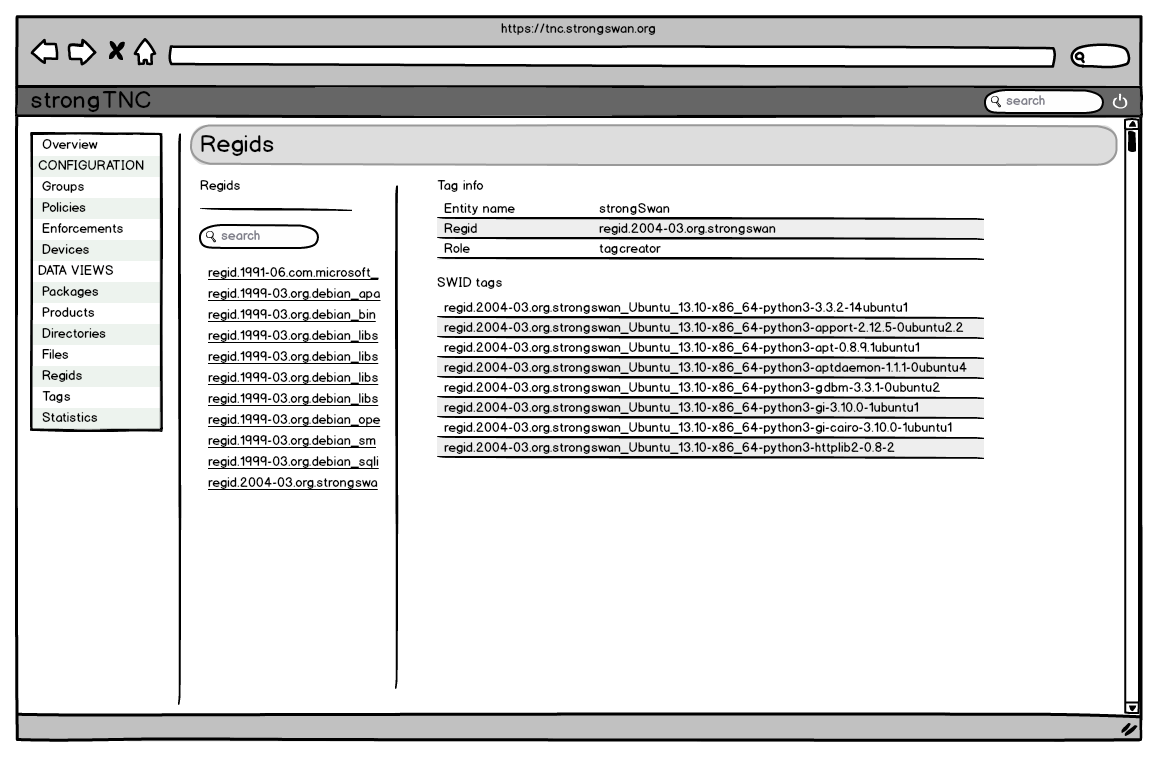
\includegraphics[width=0.8\textwidth]{./images/mockups/swid-regid-view}
\caption{Mockup Regid View.}
\label{fig:swid-regid-view}
\end{figure}
\begin{figure}[H]
\centering
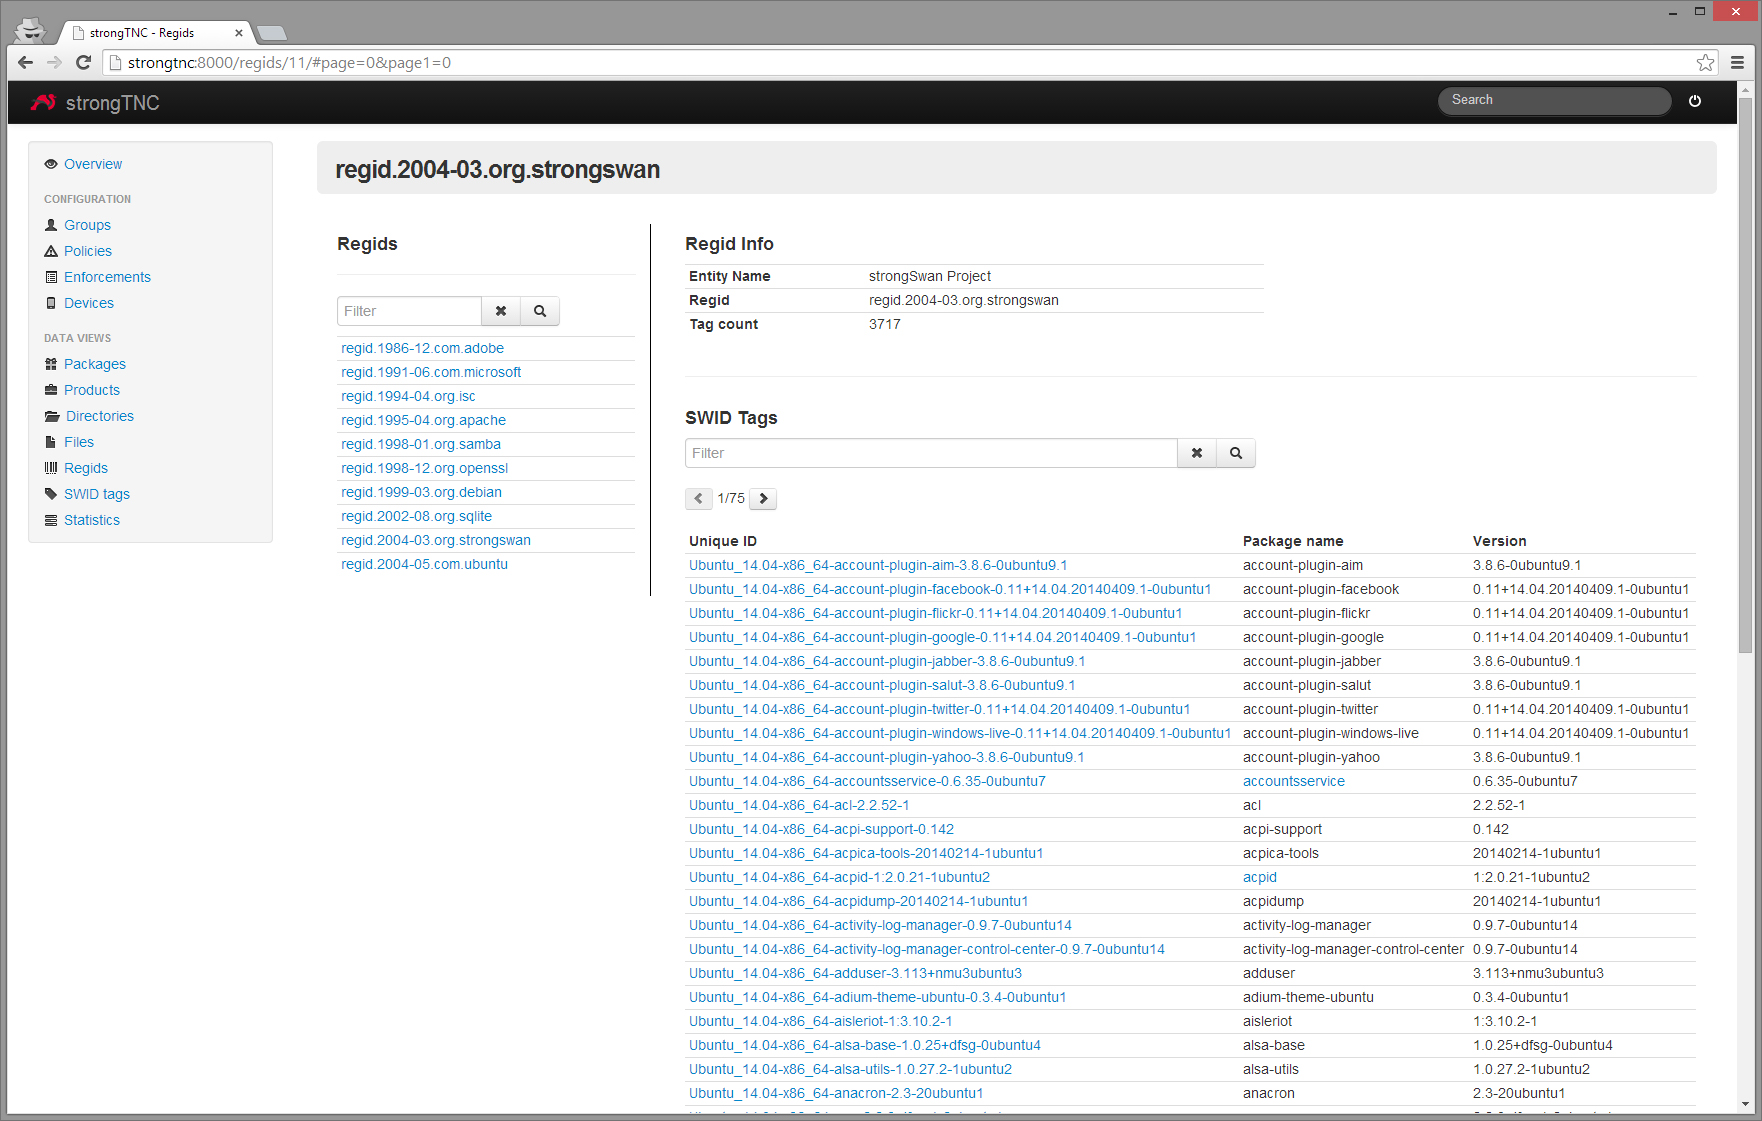
\includegraphics[width=0.8\textwidth]{./images/Views/regid-view}
\caption{Regid View mit Detailansicht}
\label{fig:regid-view}
\end{figure}

\subsubsection{SWID Tag View}
Der Zweck der SWID Tag Ansicht ist das Auflisten im System vorhandener SWID Tags (\nameref{strongTNC:UC04}).
Beim wählen eines SWID Tags werden Detailinformationen angezeigt.

\begin{figure}[H]
\centering
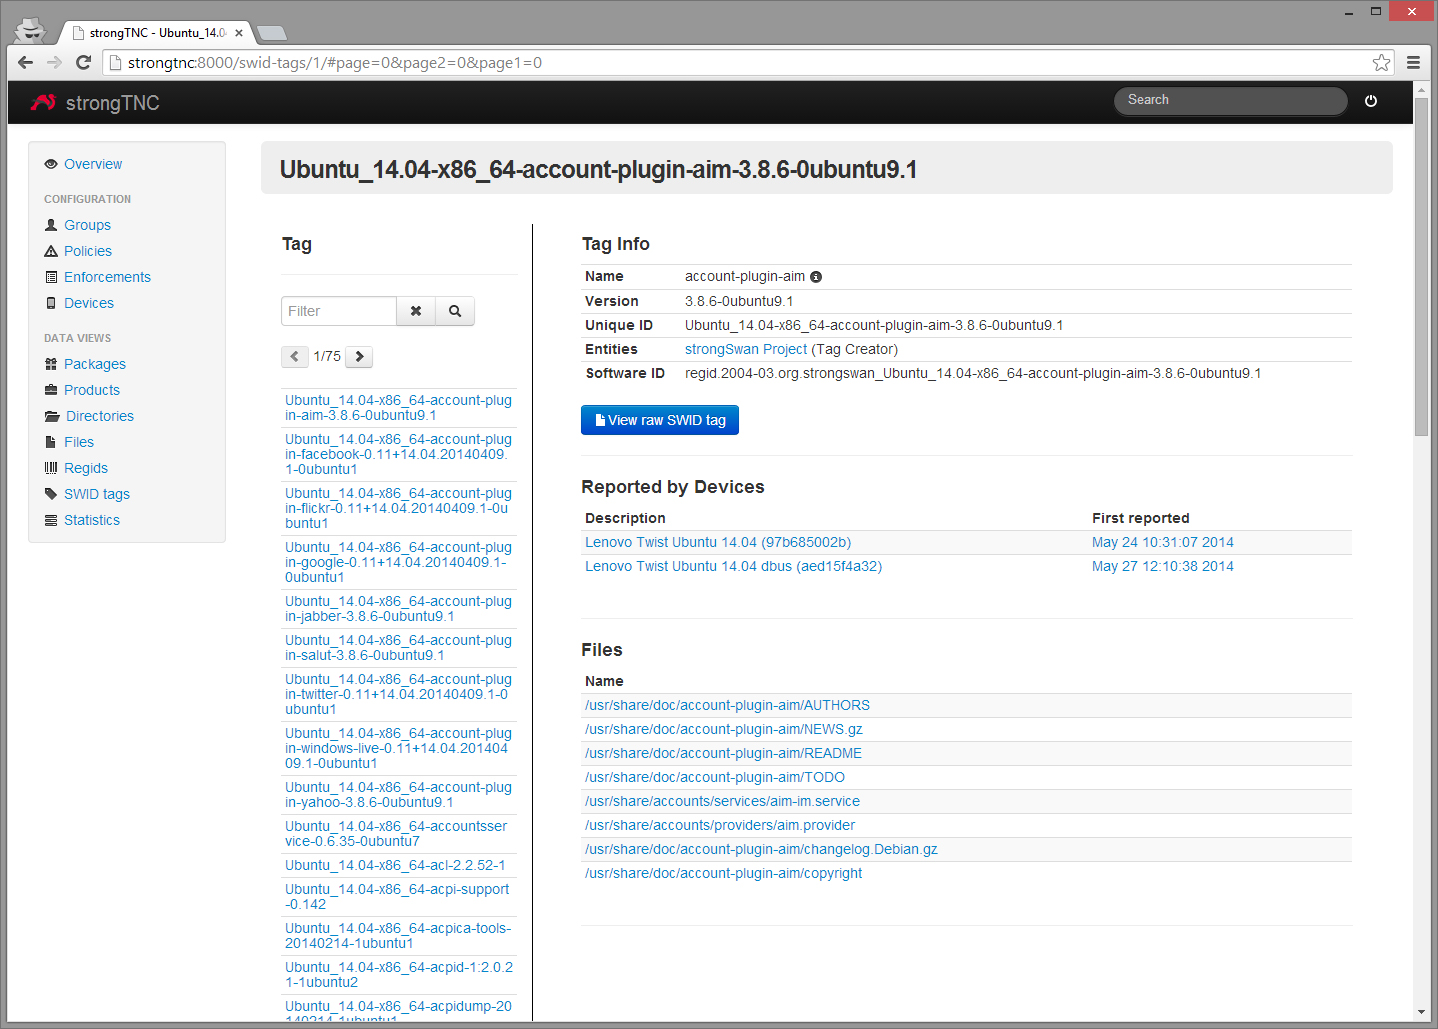
\includegraphics[width=0.8\textwidth]{./images/Views/tag-detail-view}
\caption{SWID Tag View mit Anzeige detaillierter Tag Informationen}
\label{fig:tag-detail-view}
\end{figure}

\subsubsection{SWID Inventory View}

Anhand der SWID Inventory View kann festgestellt werden, welche Software für eine ausgewählte Sitzung (Session) auf einem Gerät installiert war (\nameref{strongTNC:UC01}).

\begin{figure}[H]
\centering
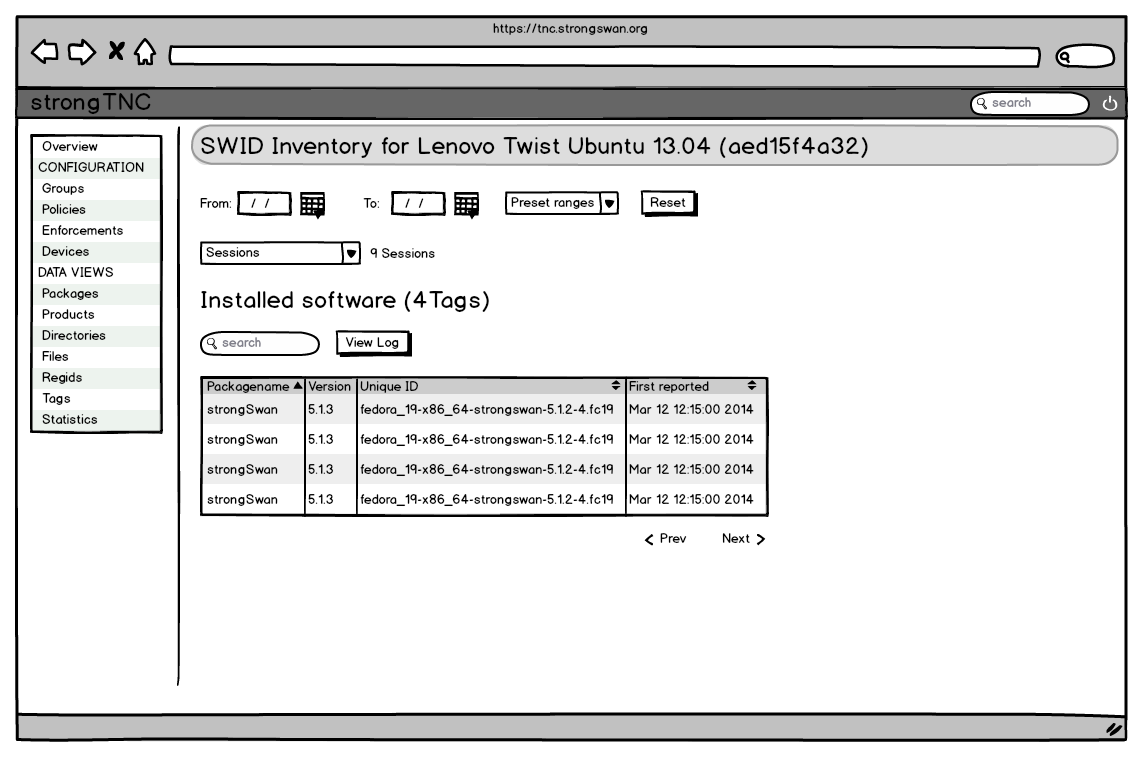
\includegraphics[width=0.8\textwidth]{./images/mockups/swid-inventory}
\caption{}
\label{fig:swid-inventory}
\end{figure}

\begin{figure}[H]
\centering
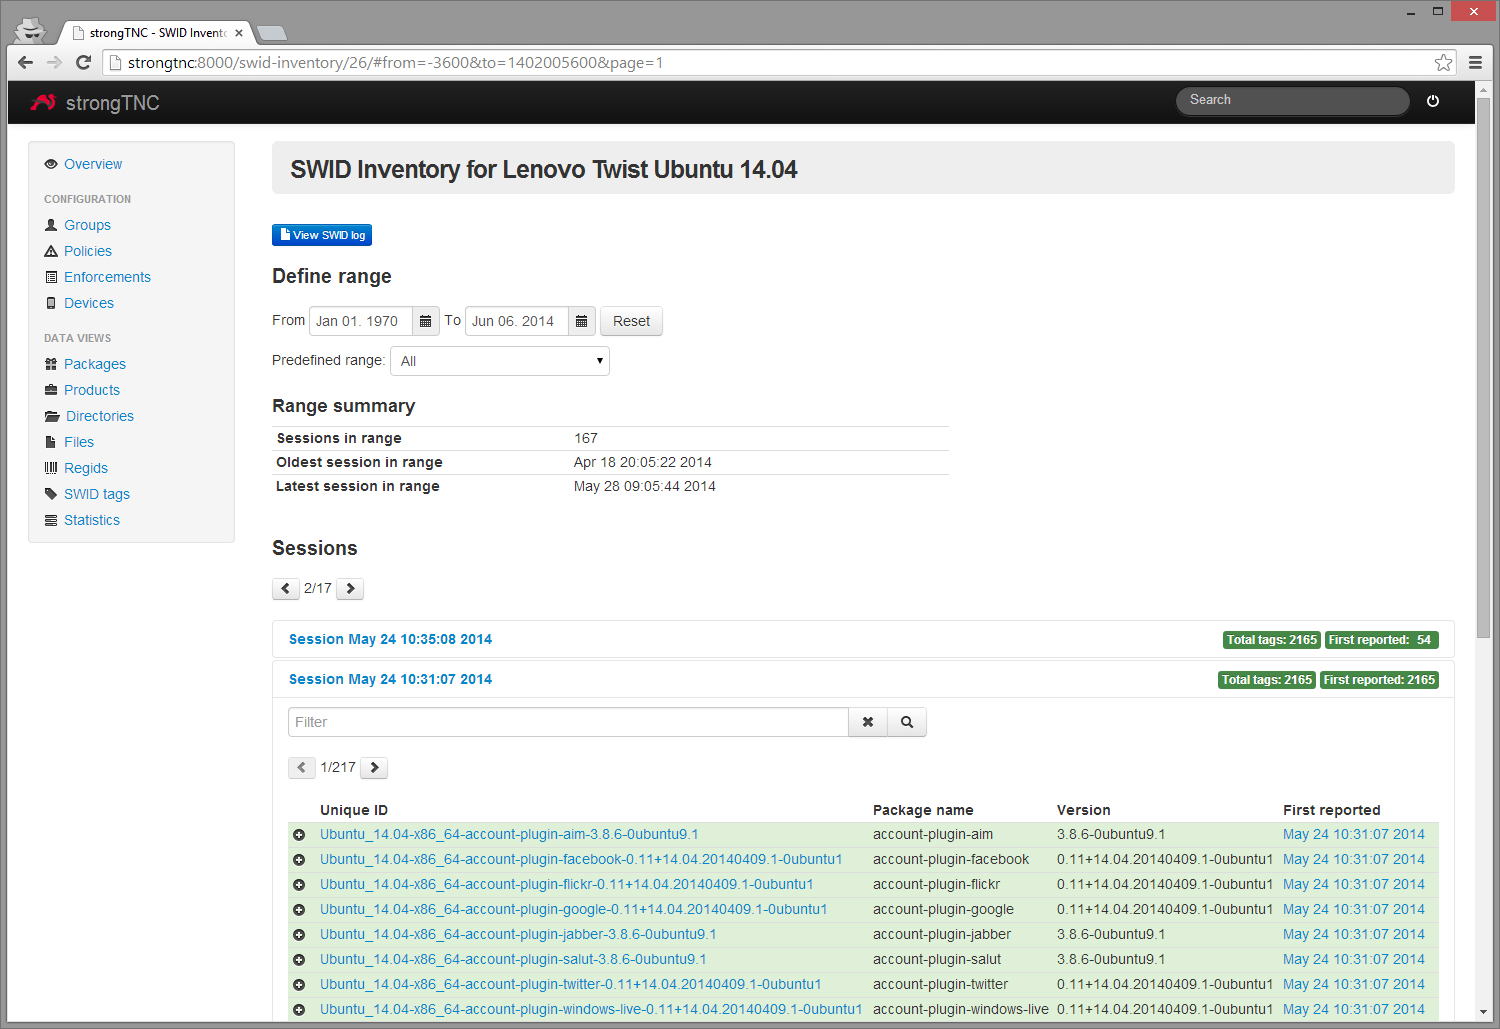
\includegraphics[width=0.8\textwidth]{./images/Views/inventory-view}
\caption{SWID Inventory View}
\label{fig:tag-detail-view}
\end{figure}


\subsubsection{SWID Log View}

Die Log View zeigt den Verlauf der Installation und Entfernung von Software Paketen auf
einem ausgewählten Gerät (\nameref{strongTNC:UC01}). Da bei jeder SWID Tag Messung jeweils alle
vorhanden SWID Tags übermittelt werden, lässt sich für jedes Paket sagen, wann
es installiert, beziehungsweise entfernt wurde. 

\begin{figure}[H]
\centering
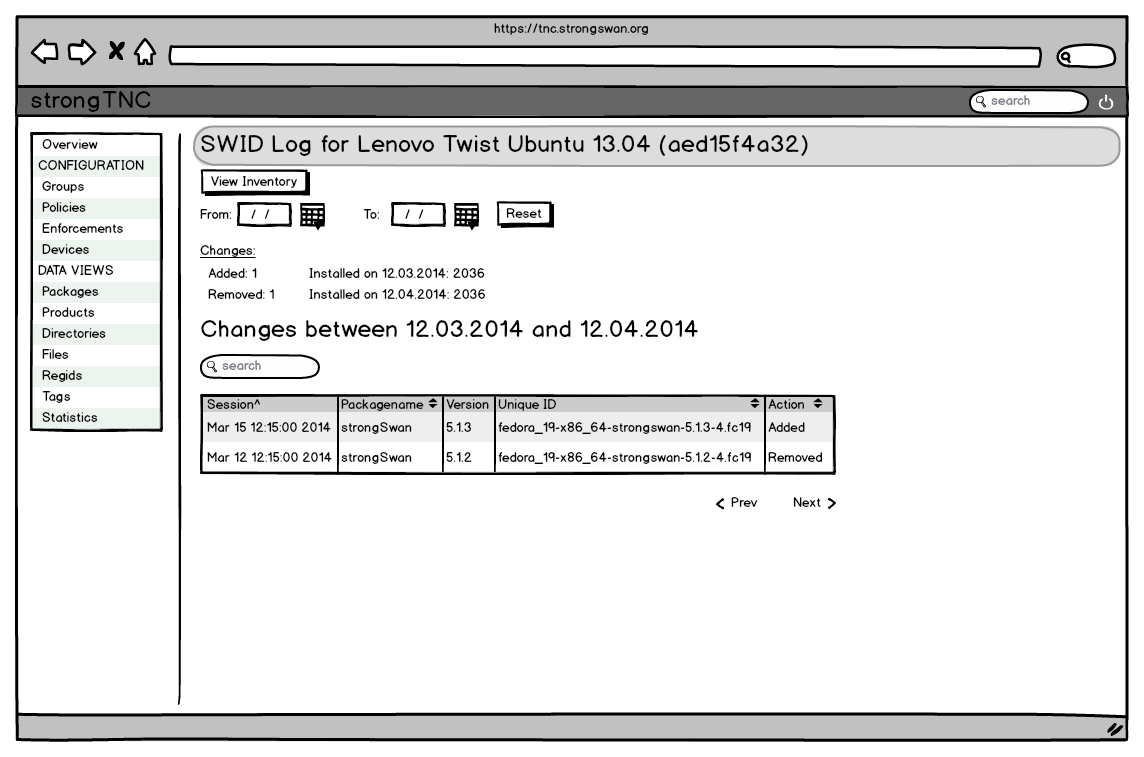
\includegraphics[width=0.8\textwidth]{./images/mockups/swid-log}
\caption{SWID Log View Mockup}
\label{fig:swid-log}
\end{figure}

\begin{figure}[H]
\centering
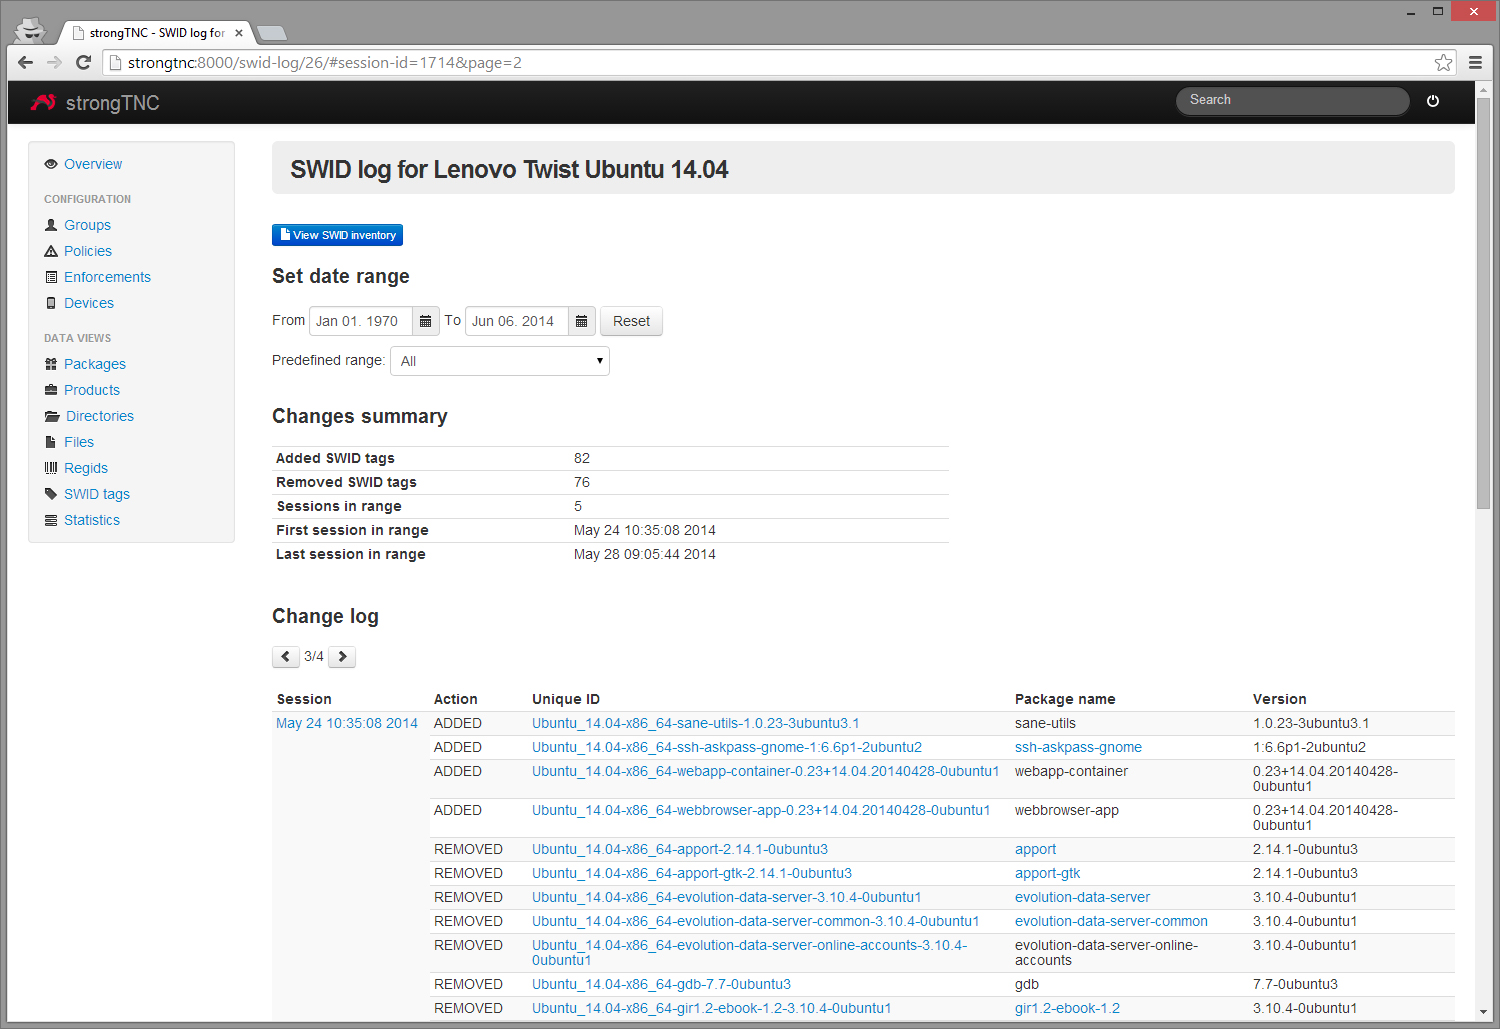
\includegraphics[width=0.8\textwidth]{./images/Views/log-view}
\caption{SWID Log View mit Details für eine ausgewählte Session}
\label{fig:log-view}
\end{figure}